\subsection{Регресионный анализ}
\label{sec:analysis:regression}

В статистическом моделировании регрессионный анализ -- это набор статистических процедур для изучения зависимостей между
случайными переменными. Он включает в себя множество методов моделирования и анализа взаимосвязей между зависимой
переменной и одной или несколькими независимыми переменными, называемых также предикторами или регрессорами.

Регрессионный анализ помогает понять, как значение зависимой переменной изменяется при изменении одной из независимых
переменных, в то время как другие независимые переменные остаются фиксированными.

Чаще всего в регрессионном анализе оценивает условное математическое ожидание зависимой переменной с учетом значений,
принимаемых независимыми переменными. Во всех случаях оцениваться функция математического ожидания зависимой переменной
от независимых переменных, называемая функцией регрессии.

Регрессионный анализ широко используется для численного предсказания, классификации и прогнозирования, где его
применение существенно перекрывается с областью машинного обучения.

В настоящее время разработано много методов регрессионного анализа. Наиболее популярными из них являются простая и
множественная линейная регрессия, среднеквадратическая и логистическая регрессия. Эти модели, являются параметрическими
в том смысле, что функция регрессии определяется конечным числом неизвестных параметров, которые оцениваются на основе данных.

В математической статистике линейная регрессия представляет собой метод аппроксимации зависимостей между входными и
выходными переменными на основе линейной модели. Является частью более широкой статистической методики, называемой
регрессионным анализом.

В регрессионном анализе входные (независимые) переменные называются также предикторными переменными или регрессорами,
а зависимые переменные — критериальными.

Если рассматривается зависимость между одной входной и одной выходной переменными, то имеет место простая линейная
регрессия. Для этого определяется уравнение регрессии 
и строится соответствующая прямая, известная как линия регрессии(рис.~\ref{fig:analysis:linear-regression}).
\begin{equation}
	\text{y} = \text{ax} + \text{b}
\end{equation}

\begin{figure}[!ht]
  \centering
  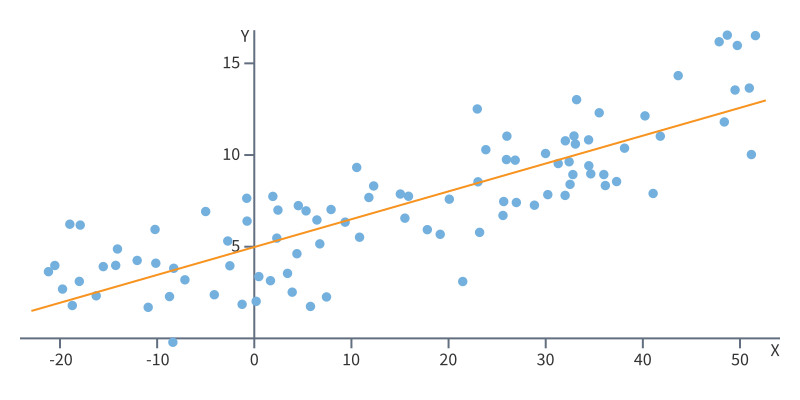
\includegraphics[scale=0.6]{linear-regression.png} 
  \caption{Линия регрессии}
  \label{fig:analysis:linear-regression}
\end{figure}

Коэффициенты \emph{a} и \emph{b}, называемые также параметрами модели, определяются таким образом, чтобы сумма квадратов
отклонений точек, соответствующих реальным наблюдениям данных, от линии регрессии была бы минимальной.
Коэффициенты обычно оцениваются методом наименьших квадратов.

Метод наименьших квадратов (МНК) — математический подход для оценки параметров моделей (например, регрессионной) на
основании экспериментальных данных, содержащих случайные ошибки.

Если данные известны с некоторой погрешностью, то вместо неизвестного точного значения параметра модели используется
приближенное. Поэтому параметры модели должны быть рассчитаны так, чтобы минимизировать разницу между экспериментальными
данными и теоретическими (вычисленными при помощи предложенной модели).

Мерой рассогласования между фактическими значениями и значениями, оцененными моделью в методе наименьших квадратов,
служит сумма квадратов разностей между ними, т.е.:

\begin{equation}
	\sum_{i=1}^{N}(\text{y}{'} - \text{y})^{2}
\end{equation}
\begin{explanation}
  где & $ \text{y}{'} $ & оценка, полученная с помощью модели;\\
  & $ \text{y} $ & фактическое наблюдаемое значение. \\
\end{explanation}

Очевидно, что лучшей будет та модель, которая минимизирует данную сумму.

Важнейшим применением МНК в анализе данных является линейная регрессия, где параметры регрессионной модели вычисляются
таким образом, чтобы сумма квадратов расстояний от линии регрессии до фактических значений данных была
минимальной~\cite{least_squares_method}.

Если ищется зависимость между несколькими входными и одной выходной переменными, то имеет место множественная линейная
регрессия. Соответствующее уравнение имеет вид:

\begin{equation}
	\text{Y} = \text{b}_{0} + \text{b}_{1}\text{x}_{1} + \text{b}_{2}\text{x}_{2} + \cdots + \text{b}_{n}\text{x}_{n}
\end{equation}
\begin{explanation}
  где & $ \text{n} $ & число входных переменных.\\
\end{explanation}

Очевидно, что в данном случае модель будет описываться не прямой, а гиперплоскостью. Коэффициенты уравнения
множественной линейной регрессии подбираются так, чтобы минимизировать сумму квадратов отклонения реальных точек данных
от этой гиперплоскости.

Преимущество множественной линейной регрессии по сравнению с простой заключается в том, что использование в модели
нескольких входных переменных позволяет увеличить долю объяснённой дисперсии выходной переменной, и таким образом
улучшить соответствие модели данным. Т.е. при добавлении в модель каждой новой переменной коэффициент детерминации растёт.

Коэффициент детерминации -- Статистический показатель, отражающий объясняющую способность регрессии \emph{a:X -> Y} и
равный отношению суммы квадратов регрессии SSR к общей вариации SST:

\begin{equation}
	\text{r}^{2} = \frac{SSR}{SST} = \frac{\sum_{i}(\text{a}(\text{x}_{i}) - \bar{y})^2}{\sum_{i}(\text{y}_{i} - \bar{y})^2} 
\end{equation}
\begin{explanation}
  где & $ \text{x}_{l}=(\text{x}_{i}, \text{y}_{i})^{l}_{i=1} $ & набор данных из \emph{l} наблюдений.\\
  & $ \text{x}_{i} $ & вектор признаков \emph{i}-го наблюдения, \\
  & $ \text{y}_{i} \in \text{Y} $ & $\text{y}_{i}$ принадлежит \emph{Y};\\ 
\end{explanation}

Данный показатель является статистической мерой согласия, с помощью которой можно определить, насколько уравнение
регрессии соответствует реальным данным.

Коэффициент детерминации изменяется в диапазоне от 0 до 1. Если он равен 0, это означает, что связь между переменными
регрессионной модели отсутствует и вместо нее для оценки значения выходной переменной можно использовать простое
среднее ее наблюдаемых значений. Напротив, если коэффициент детерминации равен 1, это соответствует идеальной модели,
когда все точки наблюдений лежат точно на линии регрессии, т.е. сумма квадратов их отклонений равна 0.

На практике, если коэффициент детерминации близок к 1, это указывает на то, что модель работает очень хорошо
(имеет высокую значимость), а если к 0, то это означает низкую значимость модели, когда входная переменная плохо
«объясняет» поведение выходной, т.е. линейная зависимость между ними отсутствует. Очевидно, что такая модель будет иметь
низкую эффективность.

В некоторых случаях коэффициент детерминации может принимать небольшие отрицательные значения, если модель получилась
«бесполезной» и ее предсказания хуже, чем оценки на основе среднего значения~\cite{coefficient_of_determination}.

Линейная регрессия была первым видом регрессионного анализа, который был тщательно изучен и начал широко использоваться
в практических приложениях. Это связано с тем, что в линейных моделях оценивание параметров проще, а также с тем,
что статистические свойства полученных оценок легче определить.

Линейная регрессия имеет много практических применений. Большинство приложений попадают в одну из двух широких категорий:
\begin{itemize}
	\item Если целью является прогнозирование, линейную регрессию можно использовать для подгонки модели к наблюдаемому набору данных.
	\item Если цель заключается в том, чтобы объяснить изменчивость выходной переменной, можно применить линейный регрессионный анализ для количественной оценки силы взаимосвязи между выходной и входными переменными.
\end{itemize}

Среднеквадратическая регрессия -- разновидность регрессии, где при определении параметров модели используется обобщение 
метода наименьших квадратов (МНК) -- метод наименьших средних квадратов.

Иными словами, в процессе подгонки модели к данным минимизируется не сумма квадратов остатков регрессии, а их средний квадрат:

\begin{equation}
	\text{E}[(\text{Y} - \text{F}(\text{X}))^{2}]
\end{equation}
\begin{explanation}
  где & $ \text{E} $ & операция усреднения,\\
  & $ \text{Y} $ & зависимая переменная, \\
  & $ \text{X} $ & вектор независимых переменных.\\ 
\end{explanation}

Это становится возможным благодаря тому, что МНК допускает широкое обобщение, когда вместо минимизации суммы квадратов
остатков можно минимизировать их некоторую положительно определённую квадратичную форму.

Смысл данного подхода заключается в том, что к результатам классического МНК (т.е. квадратам остатков) применяется
дополнительное линейное преобразование - усреднение. Как известно, одним из предположений регрессии является
предположение о нормальности остатков, которое в практических случаях не соблюдается. Усреднение позволяет снизить
степень влияния отклонения остатков от нормального распределения на качество построенной модели.

Метод наименьших средних квадратов был сформулирован Бернардом Уидроу и Тедом Хоффом в 1960 году и применён при
обучении нейронных сетей с помощью алгоритма обратного распространения ошибки.

В математическом и статистическом моделировании зависимой (выходной) называется переменная модели, которая зависит от входных
переменных и случайных факторов, воздействующих на моделируемый процесс или объект.

Выходная переменная представляет результаты работы модели. Она изменяется (варьирует) под воздействием изменения
входной переменной и случайных факторов. Изучение изменчивости выходной переменной при изменении входной и является
целью моделирования.

В статистическом моделировании и машинном обучении независимой (входной) переменной называют величину, от которой зависит
изменение выходной переменной, при этом целью построения модели является аппроксимация этой зависимости.

Аппроксимация -- математический метод, в основе которого лежит замена одних математических объектов другими, близкими к
исходным в том или ином смысле, но более простыми.~\cite{approximation}

Аппроксимация позволяет исследовать числовые характеристики и качественные свойства объекта, сводя задачу к изучению
более простых или более удобных объектов (например, тех, параметры которых легко вычисляются или известны заранее).

Например, в линейной регрессии некоторая неизвестная функция, описывающая реальные наблюдения, аппроксимируется
уравнением прямой, а если наблюдаемые данные носят нелинейный характер, то полиномами и т.д.

моделью, которая использует логистическую функцию для моделирования зависимости выходной переменной от набора входных
в случае, когда первая является бинарной.

Это разновидность множественной регрессии, общее назначение которой состоит в анализе связи между несколькими
независимыми переменными (называемыми также регрессорами или предикторами) и зависимой переменной. Регрессия в общем
виде применяется, когда входные и выходная переменные непрерывные. А логистическая регрессия лучшим образом подходит,
когда выходная переменная принимает только два значения.

Важность логистический регрессии обусловлена тем, что многие задачи анализа данных могут быть решены с помощью бинарной
классификации или сведены к ней.

Например, с помощью логистической регрессии можно оценивать вероятность наступления (или не наступления) некоторого
события: пациент болен (здоров), заемщик вернул кредит (допустил просрочку) и т.д. Благодаря этому логистическую
регрессию можно рассматривать как мощный инструмент поддержки принятия решений.

Как известно, все регрессионные модели могут быть записаны в виде формулы:

\begin{equation}
	{y} =  {F}({x}_{1}, {x}_{2}, \cdots, {x}_{n})
\end{equation}

Например, если рассматривается исход по займу, задается переменная \emph{y} со значениями 1 и 0, где 1 означает,
что соответствующий заемщик расплатился по кредиту, а 0 — что имел место дефолт.

Однако здесь возникает проблема: множественная регрессия не «знает», что переменная отклика бинарная по своей природе.
Это неизбежно приведет к модели с предсказываемыми значениями большими 1 и меньшими 0. Но такие значения вообще не
допустимы для первоначальной задачи. Таким образом, множественная регрессия просто игнорирует ограничения на диапазон
значений для \emph{y}.

Для решения проблемы задача регрессии может быть сформулирована иначе: вместо предсказания бинарной переменной мы
предсказываем непрерывную переменную со значениями на отрезке [0,1] при любых значениях независимых переменных.
Это достигается применением следующего регрессионного уравнения (логит-преобразование):

\begin{equation}
	{p} =  \frac{1}{1+e^{-y}}
\end{equation}
\begin{explanation}
  где & $ p $ & вероятность того, что произойдет интересующее событие,\\
  & $ e $ & основание натуральных логарифмов 2,71…, \\
  & $ y $ & стандартное уравнение регрессии.\\ 
\end{explanation}

Зависимость, связывающая вероятность события и величину \emph{y}, показана на следующем графике:

\begin{figure}[!ht]
  \centering
  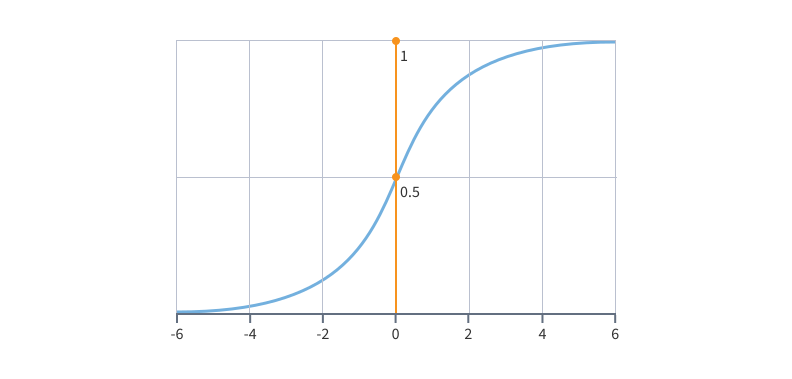
\includegraphics[scale=0.6]{logistic-regression.png} 
  \caption{Зависимость, связывающая вероятность события и величину \emph{y}}
  \label{fig:analysis:logistic-regression}
\end{figure}

Преобразование вида:

\begin{equation}
	{P'} =  \text{log}_{e}(\frac{P}{1-P})
\end{equation}

называют логистическим, или логит-преобразованием.

Существует несколько способов нахождения коэффициентов логистической регрессии. На практике часто используют метод
максимального правдоподобия. Он применяется в статистике для получения оценок параметров генеральной совокупности по
выборочным данным.

Логистическая регрессия является традиционным статистическим инструментом для расчета коэффициентов (баллов) скоринговой
карты на основе накопленной кредитной истории.

Генеральная совокупность — это совокупность всех объектов или наблюдений, относительно которых исследователь намерен
делать выводы при решении конкретной задачи. В ее состав включаются все объекты, которые подлежат изучению.

Объем генеральной совокупности может быть очень велик, и на практике рассмотреть все ее элементы не представляется
возможным. Поэтому обычно из генеральной совокупности извлекаются выборки, на основе анализа которых аналитик пытается
сделать вывод о свойствах всей совокупности, скрытых в ней закономерностях, действующих правилах и т.д. При этом выборки
должны быть репрезентативными.

Регрессионный анализ является одним из наиболее распространенных методов обработки результатов экспериментов при
изучении зависимостей в естественных науках, экономике, технике и др. областях.

В аналитических технологиях Data Mining элементы регрессионного анализа широко используются для решения задач
прогнозирования, оценивания, классификации, выявления зависимостей между признаками.

Основы регрессионного анализа были заложены А. Лежандром и Карлом Гауссом в их работах по методу наименьших квадратов в
начале 19 в.~\cite{regression_analysis}

Исходя из проведенного анализа способов применения различных методов регрессии можно сделать вывод, что наиболее
подходящим способом для анализа процесса формирования цен на недвижимость является множественный линейный регресионный
анализ.

Данное утверждение подтверждается анализом статьи~\cite{using_regression_analysis}.

В целях оценки недвижимости может применяться либо многофакторный, либо однофакторный регрессионный анализ.
В первом случае строится множественная регрессионная модель, описывающая зависимость стоимости оцениваемого объекта от
нескольких независимых определяющих факторов, значения которых определяются из анализа рыночных данных.
Этими факторами могут быть как физические характеристики объекта (площадь, качество отделки и т.п.), так и
характеристики его местоположения (удаленность от транспортных магистралей, экологическая обстановка и т.п.).

При однофакторном регрессионном анализе рассматривается зависимость переменной – стоимости единицы сравнения – от одной
независимой (контролируемой) переменной. Значения остальных независимых переменных считаются фиксированными.
В качестве независимой переменной X обычно используется показатель «общая площадь», за зависимую переменную Y
принимается показатель «стоимость 1м кв. общей площади».

В случае, когда рассматривается зависимость между одной зависимой переменной Y и несколькими независимыми
переменными Х1, Х2, ... ,Хn говорят о множественной линейной регрессии. 
